\addcontentsline{toc}{chapter}{Appendices}

% The \appendix command resets the chapter counter, and changes the chapter numbering scheme to capital letters.
%\chapter{Appendices}
\appendix
\chapter{Dijet Binning}
\label{app:dijet_bins}

\noindent
The binning used in the di-$b$-jet analysis is:
\begin{verbatim}
203, 216, 229, 243, 257, 272, 287, 303, 319, 335, 352, 369,
387, 405, 424, 443, 462, 482, 500, 523, 544, 566, 588, 611, 
634, 657, 681, 705, 730, 755, 781, 807, 834, 861, 889, 917,
 946, 976, 1006, 1037, 1068, 1100, 1133, 1166, 1200, 1234, 
1269, 1305, 1341, 1378, 1416, 1454, 1493, 1533, 1573, 1614,
 1656, 1698, 1741, 1785, 1830, 1875, 1921, 1968, 2016, 2065, 
2114, 2164, 2215, 2267, 2320, 2374, 2429, 2485, 2542, 2600, 
2659,2719, 2780, 2842, 2905, 2969, 3034, 3100, 3167, 3235, 
3305, 3376, 3448,3521, 3596, 3672, 3749, 3827, 3907, 3988, 
4070, 4154, 4239, 4326, 4414, 4504, 4595, 4688, 4782, 4878, 
4975, 5074, 5175, 5277, 5381, 5487, 5595, 5705, 5817, 5931, 
6047, 6165, 6285, 6407, 6531, 6658, 6787, 6918, 7052, 7188, 
7326, 7467, 7610, 7756, 7904, 8055, 8208, 8364, 8523, 8685, 
8850, 9019, 9191, 9366, 9544, 9726, 9911, 10100, 10292, 
10488, 10688, 10892, 11100, 11312, 11528, 11748, 11972, 
12200, 12432, 12669, 12910, 13156
\end{verbatim}

\chapter{Single Jet Trigger Threshold~\pT~Fit}
\label{app:triggerTurnOn_fit}

The threshold jet-\pT~of a single jet trigger is defind as the jet-\pT~above
which which a single jet-trigger is on the trigger plateu.
The threshold jet-\pT~follows a linear behaviour with respect to jet-\pT,
and such a linear fit can be used to predict the thresholds jet-\pT~of a single jet trigger.

Figure~\ref{fig:triggerTurnOn_fit} shows the threshold jet-\pT~
at which a trigger is 99\% efficient with respect to a lower-\pT~benchmark trigger
as a function of the trigger-level~\pT~requirements of the single jet trigger.
A linear fit is performed, as shown by the red line.
The 1$\sigma$ error band on the fit slope is shown by the dotted lines~\cite{evt-jet_turnOnFit}.

\begin{figure}[!hbt]
    \begin{center}
        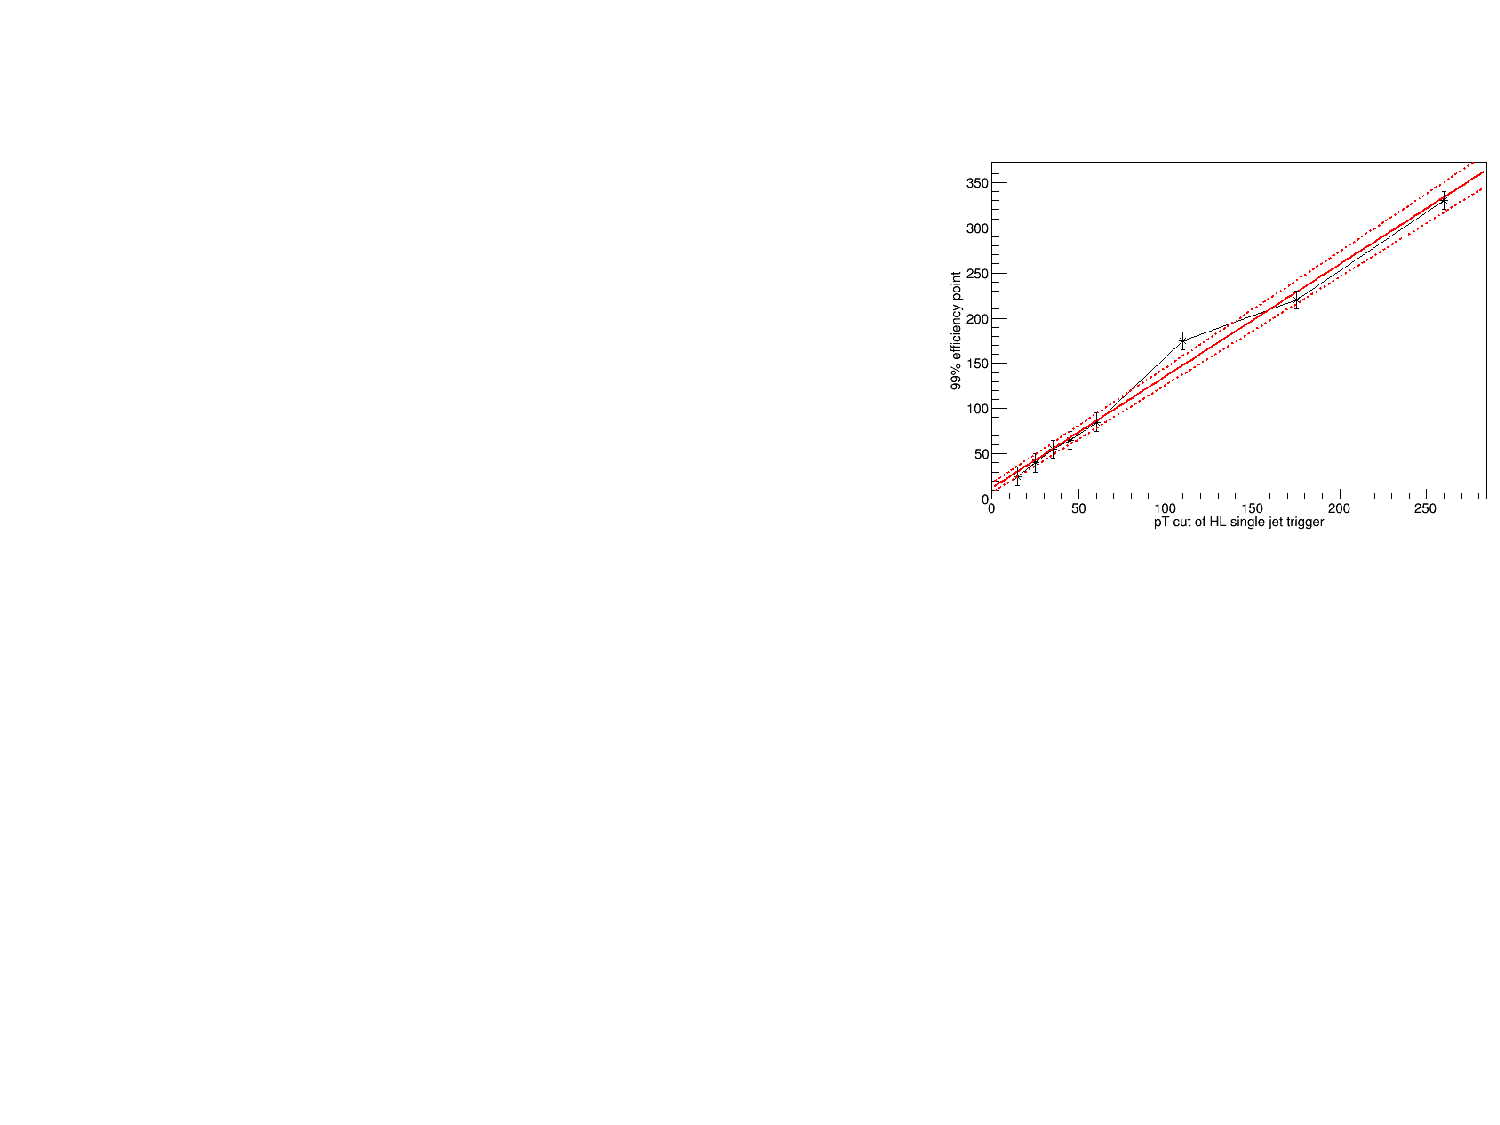
\includegraphics[width=0.6\linewidth, angle=0]{figs/Dibjet/LowMass/jetTriggerTurnOn.pdf}
      \end{center}
  \caption[A plot showing the threshold jet-\pT~at which a trigger is 99\% efficient
             with respect to a lower-\pT~benchmark trigger as a function of the trigger-level~\pT~requirements of the single jet trigger.
             A linear fit is performed, as shown by the red line. The 1$\sigma$ error band on the fit slope is shown by the dotted lines.]
           {A plot showing the threshold jet-\pT~at which a trigger is 99\% efficient
             with respect to a lower-\pT~benchmark trigger as a function of the trigger-level~\pT~requirements of the single jet trigger.
             A linear fit is performed, as shown by the red line. The 1$\sigma$ error band on the fit slope is shown by the dotted lines~\cite{evt-jet_turnOnFit}.}
          \label{fig:triggerTurnOn_fit}
\end{figure}

\noindent
The resulting linear fit has a normalisation of 12.30 and a slope of 1.236.
Using the fit for the trigger level jet requirements of the double $b$-jet trigger we obtain:
\vspace{-0.5em}
\begin{itemize}[leftmargin=*]
\item Trigger Level Jet~\pT~$>$ 150 GeV,~  Threshold Jet~\pT~$>$ 74.1 GeV 
\item Trigger Level Jet~\pT~$>$  50 GeV,~~ Threshold Jet~\pT~$>$ 197.8 GeV
\end{itemize}
\vspace{-0.3em}
\noindent
The values are rounded up in the analysis to give a safety margin.

\chapter{Colophon}
\label{appendixlabel3}
\textit{This is a description of the tools you used to make your thesis. It helps people make future documents, reminds you, and looks good.}

\textit{(example)} This document was set in the Times Roman typeface using \LaTeX\ and Bib\TeX , composed with a text editor. 
 % description of document, e.g. type faces, TeX used, TeXmaker, packages and things used for figures. Like a computational details section.
% e.g. http://tex.stackexchange.com/questions/63468/what-is-best-way-to-mention-that-a-document-has-been-typeset-with-tex#63503

% Side note:
%http://tex.stackexchange.com/questions/1319/showcase-of-beautiful-typography-done-in-tex-friends
